\documentclass[../report.tex]{subfiles}

\begin{document}

% Chapter State of the art
% - Concepts (before diving into the protocoles, it is important to understand some concepts)
% - Outlines of the KAPE landscape (all PAKEs, history, overview)
% - Mains PAKEs (differences, improvement, tableau comparatif, pas besoin de décrire les constructions)
%   - EKE
%   - SRP
%   - OPAQUE
%   - KHAPE
% - PAKE choice (and reasons)

% (Attack on PAKEs ?)


% Chapter OPAQUE or Chapter KHAPE (depending on the PAKE choice)
% - detail construction (protocol) of the choosen PAKE


\chapter{State of the art}
\section{Main PAKEs}

\subsection{OPAQUE}

% -------------------- 01 OPAQUE Paper ------------------

%%% Abstract :

% Construction :
% - "two modular constructions using an Oblivious PRF as a main tool"
%     - "builds a Strong aPAKE from any aPAKE (which in turn can be constructed from any PAKE [26])"
%     - "builds a Strong aPAKE from any authenticated key-exchange (AKE) protocol secure against KCI attacks."

% Performances :
% 3 messages
% 3 or 4 exponentiations

% Guarantees :
% - forward secrecy
% - "explicit mutual authentication"
% - PKI-free
% - "supports user-side password hardening"
% - "has a built-in facility for password-based storage-and-retrieval of secrets and credentials"
% - "accommodates a user-transparent server-side threshold implementation."

%%% Introduction :
% - password are used everywhere, from the simpliest to the most sensitive app.
% - attacker is forced to "run an exhaustive offline dictionary attack to find users' passwords given a set (dictionary) of candidate passwords"
% - "Two obious disadvantages" of the classical auth method :
%    1. "the password appears in cleatext at the server during login [ref]"
%    2. "security breaks if the TLS channel is established with a compromised server's public key (a widespread concern given today's too-common PKI failures)". "PKI failures include stealing of server private keys, software that does not verify certificates correctly, users that accept invalid or suspicious certificates, certificates issued by rogue CAs, servers that share their TLS keys with others { e.g., CDN providers or security monitoring software, information (including passwords) that traverses networks in plaintext form after TLS termination; and more."


% - "password-authenticated key exchange (PAKE), was first studied by Bellovin and Merritt [7] and later formalized by Bellare et al. [6] in the game-based indistinguishability approach. Canetti et al. [15] formalized PAKE in the Universally Composable (UC) framework [14], which better captures PAKE security issues such as the use of arbitrary password distributions, the inputting of wrong passwords by the user, and the common practice of using related passwords for different services."

% -------------------- 06 Lets talk about PAKE ----------------

%%% Advantages of OPAQUE:
% - "can be implemented in any setting where Diffie-Hellman and discrete log (type) problems are hard"
% - "can be easily instantiated using efficient elliptic curves"
% - "does not reveal the salt". No pre-commutation attack
% - "works with any password hashing function"
% - "take load off the server", "use much strong security settings" like Argon2, scrypt, ... (with resource heavy parameters)
% - approx. the same amount of messages and exponentiations than SRP. "But since it can be implemented in more efficient settings, it’s likely to be a lot more efficient."
% - "security proof in a very strong model"

% - "internet draft proposal" (standard)
% - production-grade implementation ?



%%% Oblivious PRF design :
% 1. "The main problem with earlier PAKEs is the need to transmit the salt from a server to a client"
% 2. attackers can retrieve the salt to build an offline dictionary. This is what we call a pre-computation attack.
% 3. Password hash is done client-side but doesn't use the salt that the server store.
% 4. Oblivious PRF is used to calculate another salt called 'salt2'
% 5. Then the client calculate the secret key by hashing the password with the salt2
% - if the client enter an incorrect password, the output (secret key) will be very different and he won't be able to use the key for the next step 

% Guarantees :
% - client knows the password
% - server knows the salt
% - server doesn't learn password
% - client doesn't learn the salt stored on the server
% - only the client learn the secret key (the output)


%%% Key exchange design :
% - needs an authenticated key-exchange (HMQV)
% - needs two public/private keys pair. One for the server, one for the client.

% Register :
% - When a client want to register, the client generate a public/private key pair and encrypt the private key with the secret key (output of OPRF). The ciphertext (and the public key) is sent and stored in the server.
% "C = Encrypt(K, client's private_key | server's pulic_key)"

% Login :
% - When a client want to login, the server sends the stored ciphertext to the client
% - If the password entered by the client is correct, he get the correct secret key from the OPRF
% - He can then use the secret key to decrypt the ciphertext and retrieve his private key and server's public key
% - He then use these keys to run a authenticated key exchange with the server (like HMQV ?)


% ============================================================

\paragraph{Design}
Jarecki and al. \cite{}. introduce the definition of Strong aPake (SaPAKE): an aPake secure against pre-computation attacks.

They provides two modular constructions, called the OPAQUE protocol that allow to builds SaPake protocols. The first construction allow to enhance any aPake to a SaPAKE while the second allow to enhance any Authenticated Key-Exchange (AKE) protocol (that are secure against KCI attacks) to an SaPAKE.
The security of these two construction is based on Oblivious PRF (OPRF) functions \cite{}.

These functions allow for each party, namely the client and the server, to input a secret value and then the client can use the output as a key. Neither party can learn the other party's secret and the server cannot learn the output of the function.

Overall, the OPAQUE protocol allow to secure authentication from the simplest applications to the most sensitive ones.


\begin{figure}[h]
 \centering
 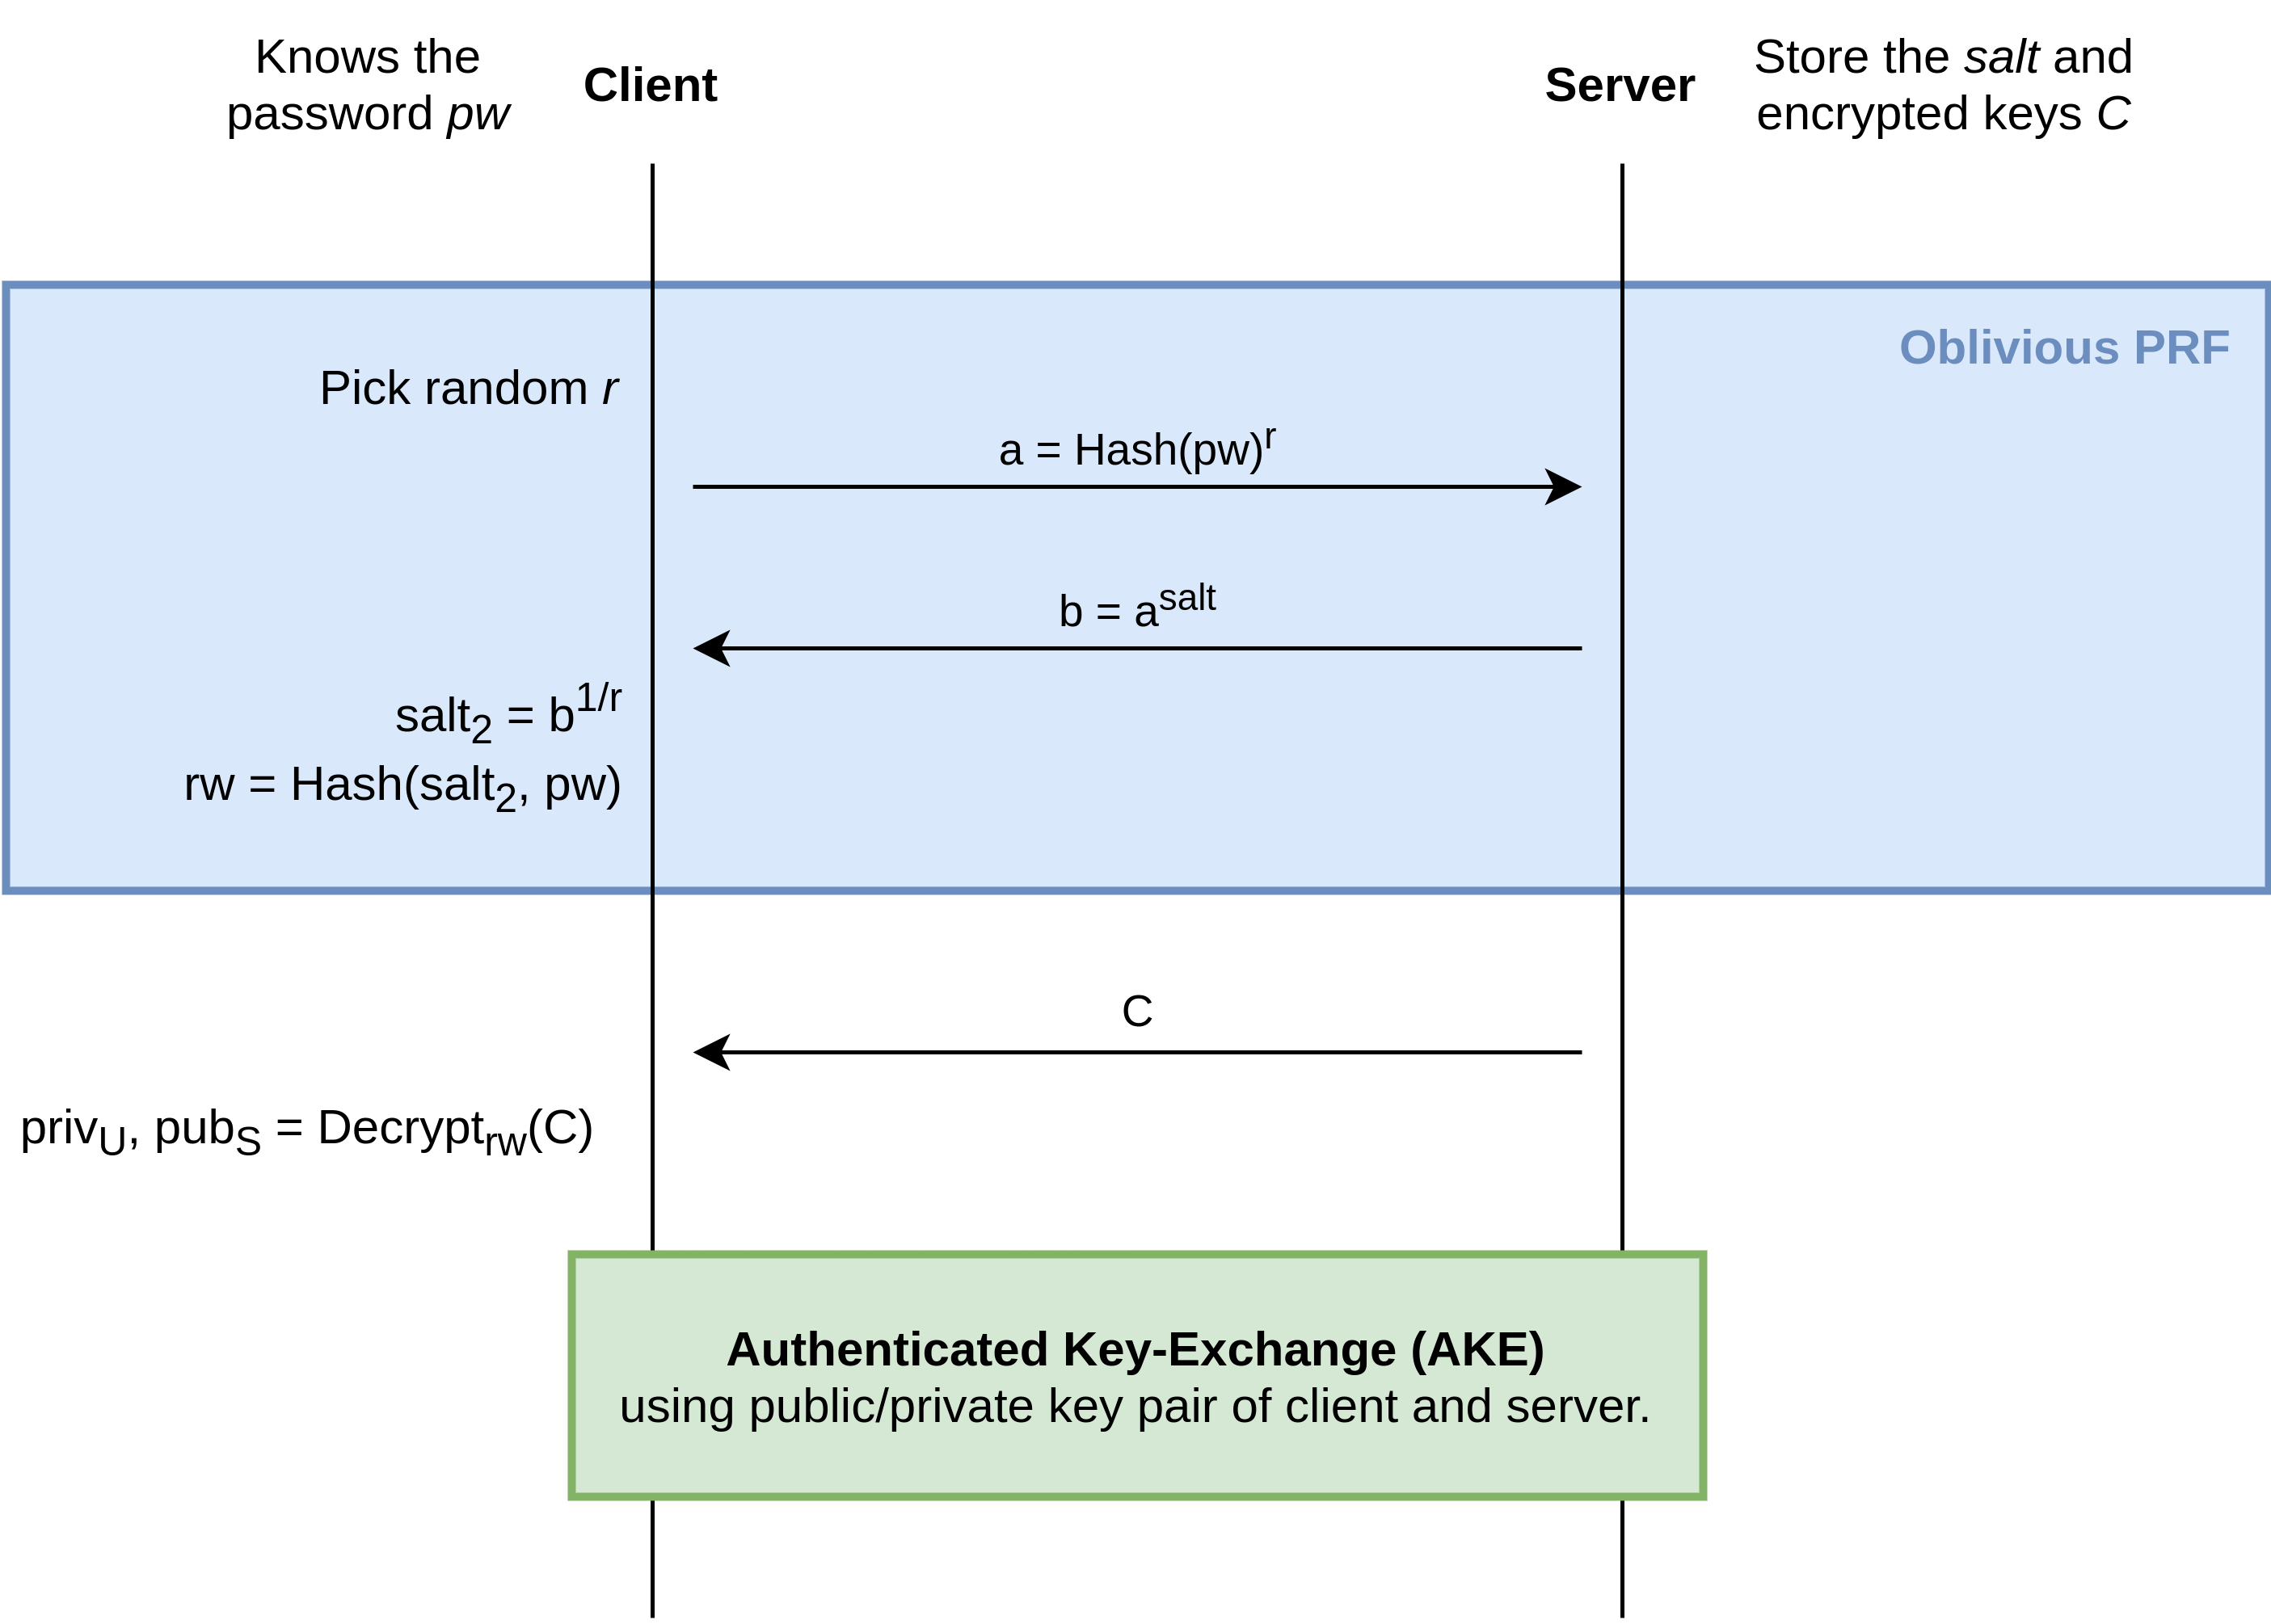
\includegraphics[width=\textwidth]{OPAQUE.png}
 % OPAQUE.png: 2166x1206 px, 72dpi, 76.41x42.54 cm, bb=0 0 2166 1206
 \caption{Login process with OPAQUE protocol using OPRF and AKE.}
 \label{fig:OPAQUE_AKE}
\end{figure}




\paragraph{Construction}

Fig \ref{fig:OPAQUE_AKE} shows the OPAQUE protocol using OPRF and AKE during login process.
The steps are the following :

(1) Generate a random value r to blind the hash of password so that the server cannot retrieve the password from the mapping.
(2) Send result to server
(3) Server add the salt to the password
(4) Client calculate the exponant of the inverse of r to unblind the value. He canno't retrieve salt.
(5) With the secret salt salt2, client compute secret key sk.
(6) Server send encrypted keys ek to clients. ek contains server's public key and client's private key encrypted with sk.
(7) If the password entered is correct, client can use sk to decrypt ek and retrieve his private key privU
(8) With both keys, clients and server can run an authenticated key exchange for mutual authentication.


\paragraph{Register}
When a client want to register, the client generate a public/private key pair. He then encrypt his private key and the server's public key with the secret key (OPRF's output).
$C = Encrypt_rw_(client's private key | server's public key)$

Then he send the ciphertext to the server to store.


\paragraph{Login}
For the login phase, the client enter it's password in the OPRF and the server send the ciphertext to the client.
If the password entered is correct, the client can decrypt the ciphertext with OPRF output to obtain his private key and the server's public key.
He then use these keys to run a authenticated key exchange with the server (like HMQV ?).

In the other hand, if the password is wrong, the OPRF output is totally different and the ciphertext decryption make the keys uncorrect and the server will refuse it during the key exchange (?). % TODO confirmation



% Login :
% - When a client want to login, the server sends the stored ciphertext to the client
% - If the password entered by the client is correct, he get the correct secret key from the OPRF
% - He can then use the secret key to decrypt the ciphertext and retrieve his private key and server's public key
% - He then use these keys to run a authenticated key exchange with the server (like HMQV ?)



\section{Comparing mains solutions}

\begin{center}
   \begin{tabular}{ | p{8cm} || c | c | c | c | c | }
     \hline
     \textbf{Criteria} & \textbf{EKE} & \textbf{SRP} & \textbf{OPAQUE} & \textbf{KHAPE} \\ \hline
     
     % Content :
     
     % Qualities (security guarantees)
     
     Avoid sending cleartext password to server (aPAKE) & x & x & Yes & x \\ \hline
     
     Secure against pre-computation attacks {"What's needed is that upon a server compromised, and the stealing of the password file, an attacker is forced to perform an exhaustive offline dictionary attack."} (SaPAKE) & x & x & Yes & x \\ \hline
     
     (Salt not sent in cleartext) & x & x & Yes & x \\ \hline
     Forward secrecy & x & x & Yes & x \\ \hline
     "Explicit mutual authentication" & x & x & Yes & x \\ \hline
     "PKI-free (registration?)" & x & x & Yes & x \\ \hline
     "supports user-side password hardening" & x & x & Yes & x \\ \hline
     "has a built-in facility for password-based storage-and-retrieval of secrets and credentials" & x & x & Yes & x \\ \hline
     "accommodates a user-transparent server-side threshold implementation" & x & x & Yes & x \\ \hline
     "far more secure alternative to the practice of deriving low-entropy secrets directly from a user's password" & x & x & Yes & x \\ \hline
     
     Vulnerable to Oblivious PRF compromise & x & x & Yes & x \\ \hline
     Internet standard & x & x & Draft & x \\ \hline
     
     "security proof in a very strong model" & x & x & Yes & x \\ \hline
     
     % Performances
     
     Easily adaptable to elliptics curves & x & x & Yes & x \\ \hline
     Number of messages & x & x & 3 ? & x \\ \hline
     Number of exponentiations & x & x & 3 or 4 ? & x \\ \hline

     \end{tabular}
 \end{center}





\end{document}
